%
% ---------------------------------------------------------------
% Copyright (C) 2012-2018 Gang Li
% ---------------------------------------------------------------
%
% This work is the default powerdot-tuliplab style test file and may be
% distributed and/or modified under the conditions of the LaTeX Project Public
% License, either version 1.3 of this license or (at your option) any later
% version. The latest version of this license is in
% http://www.latex-project.org/lppl.txt and version 1.3 or later is part of all
% distributions of LaTeX version 2003/12/01 or later.
%
% This work has the LPPL maintenance status "maintained".
%
% This Current Maintainer of this work is Gang Li.
%
%

\documentclass[
 size=14pt,
 paper=smartboard,  %a4paper, smartboard, screen
 mode=present, 		%present, handout, print
 display=slides, 	% slidesnotes, notes, slides
 style=tuliplab,  	% TULIP Lab style
 pauseslide,
 fleqn,leqno]{powerdot}


\usepackage{cancel}
\usepackage{caption}
\usepackage{stackengine}
\usepackage{smartdiagram}
\usepackage{attrib}
\usepackage{amssymb}
\usepackage{amsmath} 
\usepackage{amsthm} 
\usepackage{mathtools}
\usepackage{rotating}
\usepackage{graphicx}
\usepackage{epsfig,graphicx,subfigure}
\usepackage{boxedminipage}
\usepackage{rotate}
\usepackage{calc}
\usepackage[absolute]{textpos}
\usepackage{psfrag,overpic}
\usepackage{fouriernc}
\usepackage{pstricks,pst-3d,pst-grad,pstricks-add,pst-text,pst-node,pst-tree}
\usepackage{moreverb,epsfig,subfigure}
\usepackage{color}
\usepackage{booktabs}
\usepackage{etex}
\usepackage{breqn}
\usepackage{multirow}
\usepackage{natbib}
\usepackage{bibentry}
\usepackage{gitinfo2}
\usepackage{siunitx}
\usepackage{nicefrac}
%\usepackage{geometry}
%\geometry{verbose,letterpaper}
\usepackage{media9}
\usepackage{animate}
%\usepackage{movie15}
\usepackage{auto-pst-pdf}

\usepackage{breakurl}
\usepackage{fontawesome}
\usepackage{xcolor}
\usepackage{multicol}



\usepackage{verbatim}
\usepackage[utf8]{inputenc}
\usepackage{dtk-logos}
\usepackage{tikz}
\usepackage{adigraph}
%\usepackage{tkz-graph}
\usepackage{hyperref}
%\usepackage{ulem}
\usepackage{pgfplots}
\usepackage{verbatim}
\usepackage{fontawesome}


\usepackage{todonotes}
% \usepackage{pst-rel-points}
\usepackage{animate}
\usepackage{fontawesome}

\usepackage{listings}
\lstset{frameround=fttt,
frame=trBL,
stringstyle=\ttfamily,
backgroundcolor=\color{yellow!20},
basicstyle=\footnotesize\ttfamily}
\lstnewenvironment{code}{
\lstset{frame=single,escapeinside=`',
backgroundcolor=\color{yellow!20},
basicstyle=\footnotesize\ttfamily}
}{}


\usepackage{hyperref}
\hypersetup{ % TODO: PDF meta Data
  pdftitle={Presentation Title},
  pdfauthor={Gang Li},
  pdfpagemode={FullScreen},
  pdfborder={0 0 0}
}


% \usepackage{auto-pst-pdf}
% package to show source code

\definecolor{LightGray}{rgb}{0.9,0.9,0.9}
\newlength{\pixel}\setlength\pixel{0.000714285714\slidewidth}
\setlength{\TPHorizModule}{\slidewidth}
\setlength{\TPVertModule}{\slideheight}
\newcommand\highlight[1]{\fbox{#1}}
\newcommand\icite[1]{{\footnotesize [#1]}}

\newcommand\twotonebox[2]{\fcolorbox{pdcolor2}{pdcolor2}
{#1\vphantom{#2}}\fcolorbox{pdcolor2}{white}{#2\vphantom{#1}}}
\newcommand\twotoneboxo[2]{\fcolorbox{pdcolor2}{pdcolor2}
{#1}\fcolorbox{pdcolor2}{white}{#2}}
\newcommand\vpspace[1]{\vphantom{\vspace{#1}}}
\newcommand\hpspace[1]{\hphantom{\hspace{#1}}}
\newcommand\COMMENT[1]{}

\newcommand\placepos[3]{\hbox to\z@{\kern#1
        \raisebox{-#2}[\z@][\z@]{#3}\hss}\ignorespaces}

\renewcommand{\baselinestretch}{1.2}


\newcommand{\draftnote}[3]{
	\todo[author=#2,color=#1!30,size=\footnotesize]{\textsf{#3}}	}
% TODO: add yourself here:
%
\newcommand{\gangli}[1]{\draftnote{blue}{GLi:}{#1}}
\newcommand{\shaoni}[1]{\draftnote{green}{sn:}{#1}}
\newcommand{\gliMarker}
	{\todo[author=GLi,size=\tiny,inline,color=blue!40]
	{Gang Li has worked up to here.}}
\newcommand{\snMarker}
	{\todo[author=Sn,size=\tiny,inline,color=green!40]
	{Shaoni has worked up to here.}}

%%%%%%%%%%%%%%%%%%%%%%%%%%%%%%%%%%%%%%%%%%%%%%%%%%%%%%%%%%%%%%%%%%%%%%%%
% title
% TODO: Customize to your Own Title, Name, Address
%
\title{New York City Taxi Fare Prediction}
\author{
Runsha Pan
\\
\\Hunan University
}
\date{\gitCommitterDate}


% Customize the setting of slides
\pdsetup{
% TODO: Customize the left footer, and right footer
rf=\href{http://www.tulip.org.au}{
Last Changed by: \textsc{\gitCommitterName}\ \gitVtagn-\gitAbbrevHash\ (\gitAuthorDate)
},
cf={Group Outlying Aspects Mining},
}


\begin{document}

\maketitle

%\begin{slide}{Overview}
%\tableofcontents[content=sections]
%\end{slide}


%%==========================================================================================
%%
\begin{slide}[toc=,bm=]{Overview}
\tableofcontents[content=currentsection,type=1]
\end{slide}
%%
%%==========================================================================================


\section{Problem Description}



%%==========================================================================================
%%
\begin{slide}{Overview}
\begin{center}
\twotonebox{\rotatebox{90}{Problem}}{\parbox{.86\textwidth}
{
\begin{itemize}
\item Predicting the taxi fare according to the known features of the passengers taking taxis, which including 
longitude coordinate and latitude coordinate of where the taxi ride started and so on..
\item Do better 
than this using Machine Learning techniques: an RMSE of $5-$8
\end{itemize}
}}

\end{center}
\begin{center}
  \twotonebox{\rotatebox{90}{Evaluation}}{\parbox{.86\textwidth}
  {RMSE measures the difference between the predictions of a model, 
  and the corresponding ground truth.
  \begin{itemize}
  \item RMSE is given by:
  $$
  \textcolor{orange}{RMSE =\sqrt{\frac{1}{n}\sum_{i=1}^n (\hat{y_i}-y_i)^2}}
  $$
  \end{itemize}
  }}
\end{center}
\bigskip

%%==========================================================================================
\begin{note}
First, I will introduce the problem definition.
In the real life,
a teacher may be interested in the characteristics that
make one student obvious different from others.
Or,
NBA sports coaches would prefer to
know the advantages and disadvantages of one player.
Here, the player can be regarded as a query object.

For example, team A has five players,
each player has four features.
The NBA sports coaches may want to know the features of
player $1$ that are different from others.

The above example can be seen as outlying aspects mining.
The main purpose of outlying aspects mining is to identify
the outstanding features of the query object.
\end{note}
%%==========================================================================================

\end{slide}
%%
%%==========================================================================================

%%==========================================================================================
%%
\begin{slide}{Dataset Description}
  \begin{itemize}
  \item
  Files: train.csv; test.csv; sample_submission.csv
  \end{itemize}

  \begin{itemize}
  \item
  Data fields
    \begin{itemize}
    \item
    ID: \textcolor{orange}{key} - Comprised of pickup_datetime plus a unique integer.

    \item
    Features
      \begin{itemize}
      \item
      \textcolor{orange}{pickup_datetime} - timestamp value indicating when the taxi ride started.
      \item
      \textcolor{orange}{pickup_longitude}  - float for longitude coordinate of where the taxi ride started.
      \item
      \textcolor{orange}{pickup_latitude} - float for latitude coordinate of where the taxi ride started.
      \item
      \textcolor{orange}{dropoff_longitude} - float for longitude coordinate of where the taxi ride ended.
      \item
      \textcolor{orange}{dropoff_latitude} - float for latitude coordinate of where the taxi ride ended.
      \item
      \textcolor{orange}{passenger_count} - integer indicating the number of passengers in the taxi ride.
      \end{itemize}
    
    \item
    Target: \textcolor{orange}{fare_amount} - float dollar amount of the cost of the taxi ride. 
    \end{itemize}
  \end{itemize}
  
%%==========================================================================================
\end{slide}
%%
%%==========================================================================================











\section{Exploration and Preprocessing}


%%==========================================================================================
%%
\begin{slide}{Exploratory data analysis}
%Related Work - Outlying Aspects Mining
\begin{itemize}
\item
Data import and preliminary processing.


\begin{itemize}
  \item
  Import the data and view it.
  \item
  Calculating eigenvalues.minimum value, etc.
  \item
  Preliminary processing of date types and sorting.
  % \textcolor{orange}{Feature selection}
\end{itemize}


% \vspace{1cm}
% \twocolumn[
% \savevalue{lfrheight}=5cm,
% \savevalue{lfrprop}={
% linestyle=solid,framearc=.2,linewidth=1pt},
% rfrheight=\usevalue{lfrheight},
% rfrprop=\usevalue{lfrprop}
% ]{
% Disadvantages
% \begin{itemize}
% \item
% \smallskip
% Positive and negative classes are \textcolor{orange}{Not} balanced.

% \item
% \smallskip
% \textcolor{orange}{Not} quantify the outlying degree accurately.

% \item
% \smallskip
% \textcolor{orange}{Not} identify group outlying aspects.
% \end{itemize}
% }
% {
% Advantages
% \begin{itemize}
% \item
% \smallskip
% Easy to operate.

% \item
% \smallskip
% Resolve dimensionality bias.
% \end{itemize}
% }
\end{itemize}

\begin{itemize}
  \item
  Handling missing values.

  \begin{itemize}
    \item
    Deleting 14 rows with missing values, resulting in \textcolor{orange}{1999986} remaining rows.
    % \textcolor{orange}{Feature selection}
  \end{itemize}
\end{itemize}

\begin{itemize}
  \item
  Handling outliers.Remaining \textcolor{orange}{1999822} rows.

  \begin{itemize}
    \item
    The fare should be positive.Delete 77 lines with negative fares.
    \item
    latitude:[-90,90],longitude:[-180,180].Deleting rows outside the range.
    \item
    The number of passengers has an outlier of 208, which should be removed.
    % \textcolor{orange}{Feature selection}
  \end{itemize}
\end{itemize}

%%==========================================================================================
\begin{note}
Let me introduce two existing methods:
Feature selection and score-and-search.

For feature selection,
the query point can be regarded as positive class and
the rest of the data can be regarded as negative class,
selected the features that best distinguish the two classes.

The advantages of this method are easy to operate,
and it's able to resolve dimensionality bias.
However, it has some drawbacks.
Firstly,
positive and negative classes are Not balanced,
secondly,
it can't quantify the outlying degree correctly.
Most importantly,
it doesn't identify group outlying aspects.
\end{note}
%%==========================================================================================

\end{slide}
%%
%%==========================================================================================




%%==========================================================================================
%%
\begin{slide}{Data Visualization}
  %Step One - Group Feature Extraction}
  \begin{itemize}
  \item
  \smallskip
  Plot the passenger fare histogram.
  
  Combined with the data description results of the training set, the histogram of passenger consumption in the training set was made, and the outliers of passenger consumption were screened and removed.
  \end{itemize}
  
  \bigskip
  \bigskip
  \begin{figure}[htbp]
    \centering
    \subfigure[figure 1:100 groups]
    {
        \begin{minipage}[b]{.3\linewidth}
            \centering
            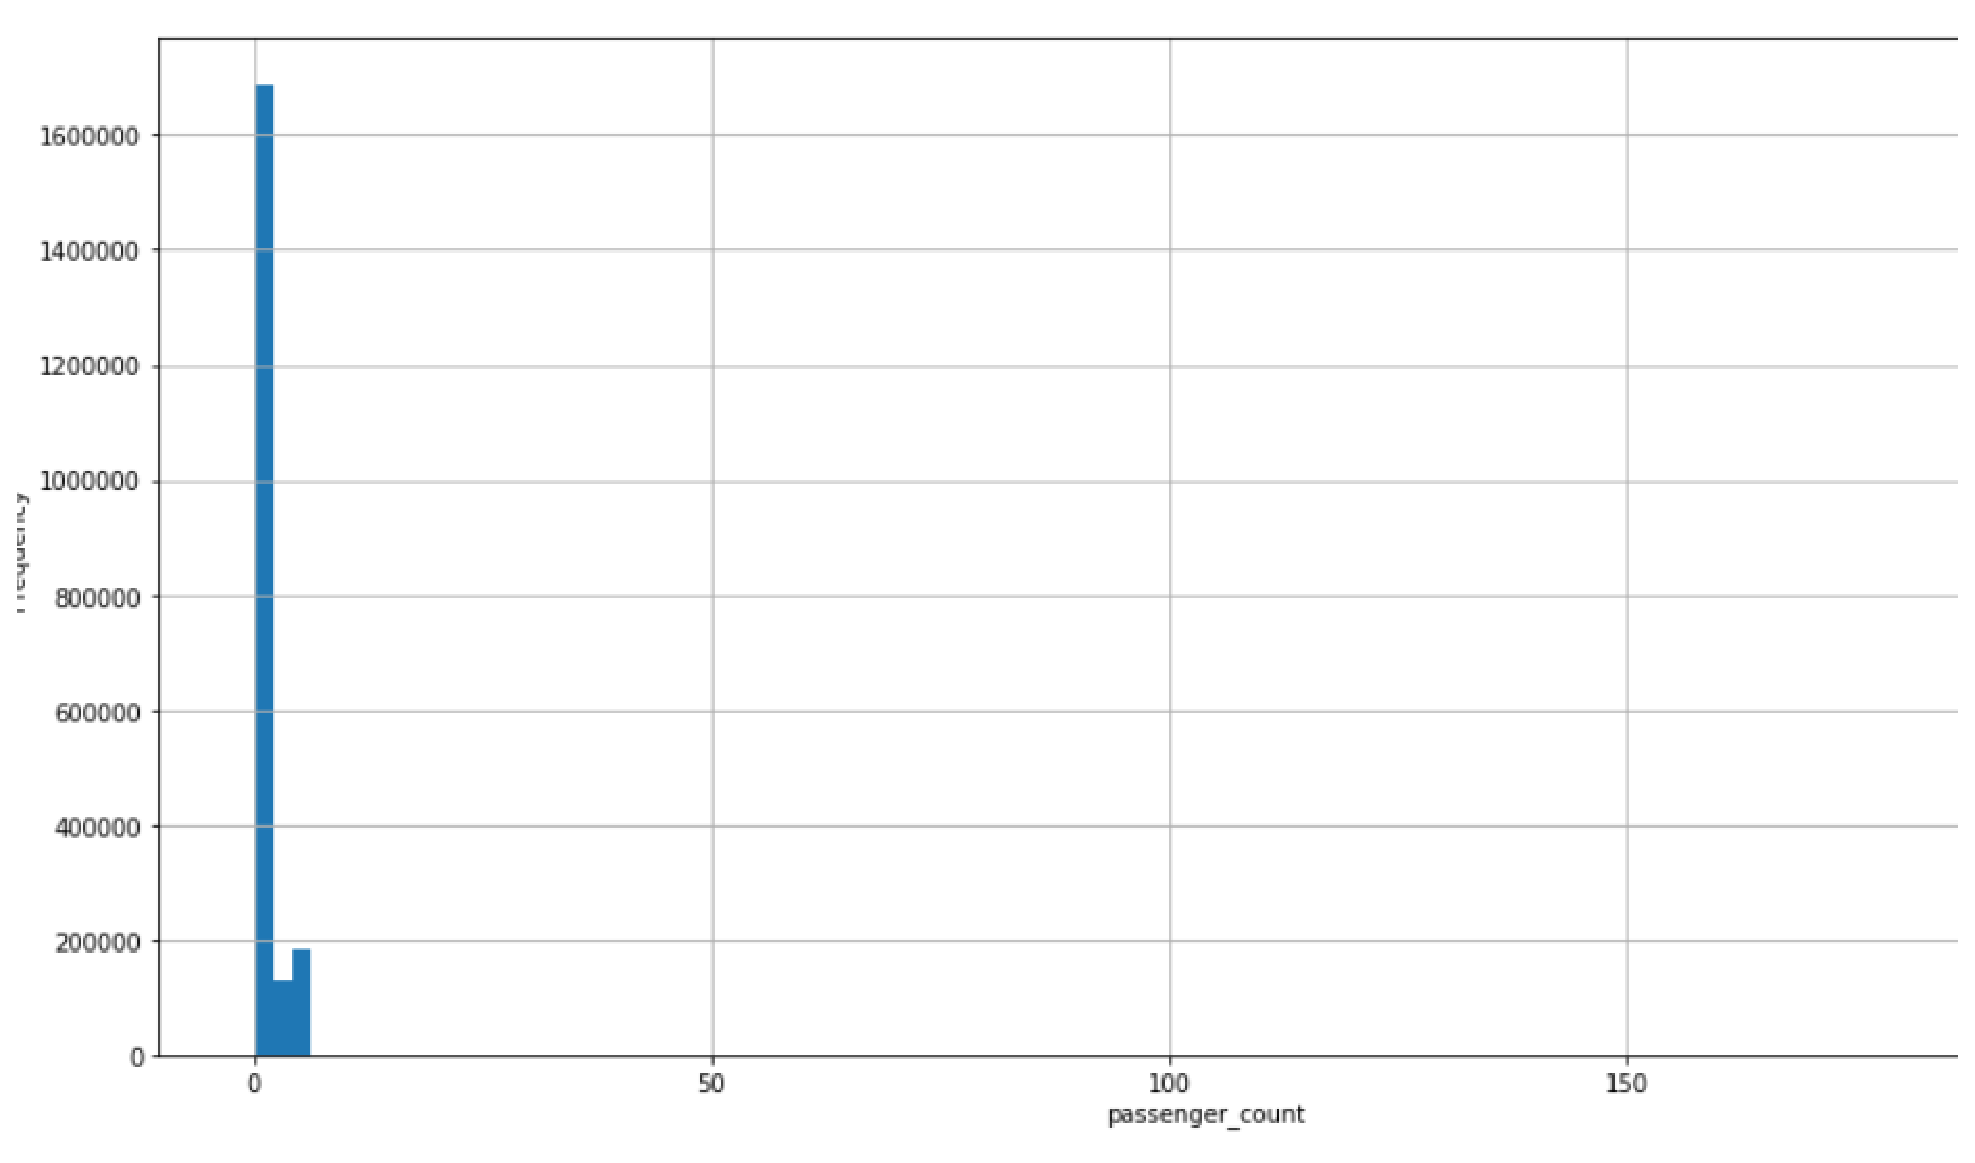
\includegraphics[scale=0.15]{01.eps}
            \label{fig:fre-dis-f3}
        \end{minipage}
    }
    \subfigure[figure 2:10 groups,x<10]
    {
       \begin{minipage}[b]{.3\linewidth}
            \centering
            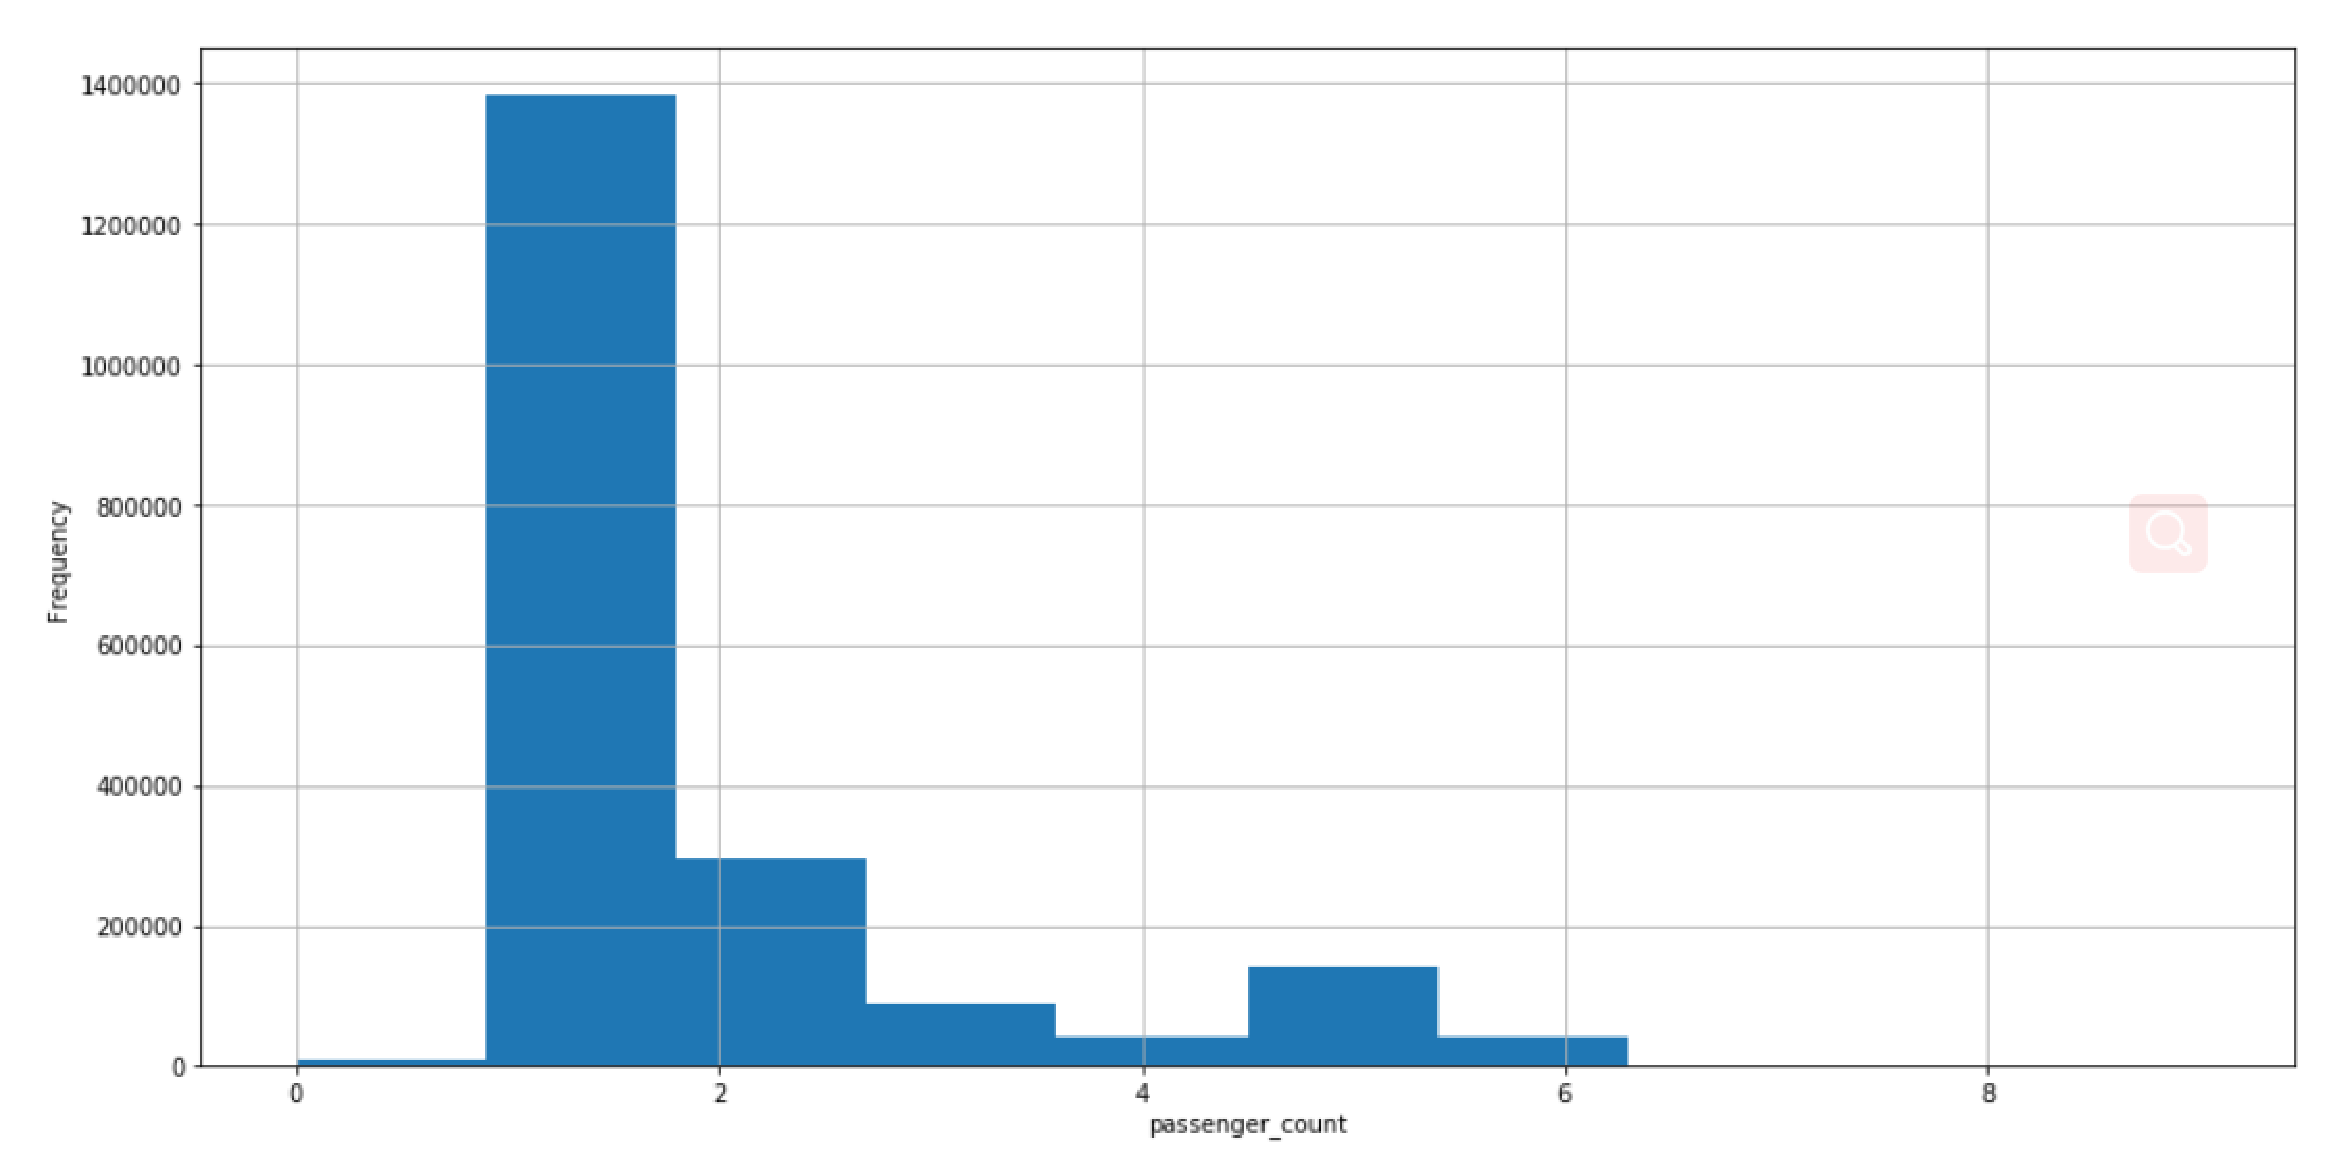
\includegraphics[scale=0.15]{2.eps}
        \end{minipage}
    }
    \subfigure[figure 3:10 groups,x>=10]
    {
       \begin{minipage}[b]{.3\linewidth}
            \centering
            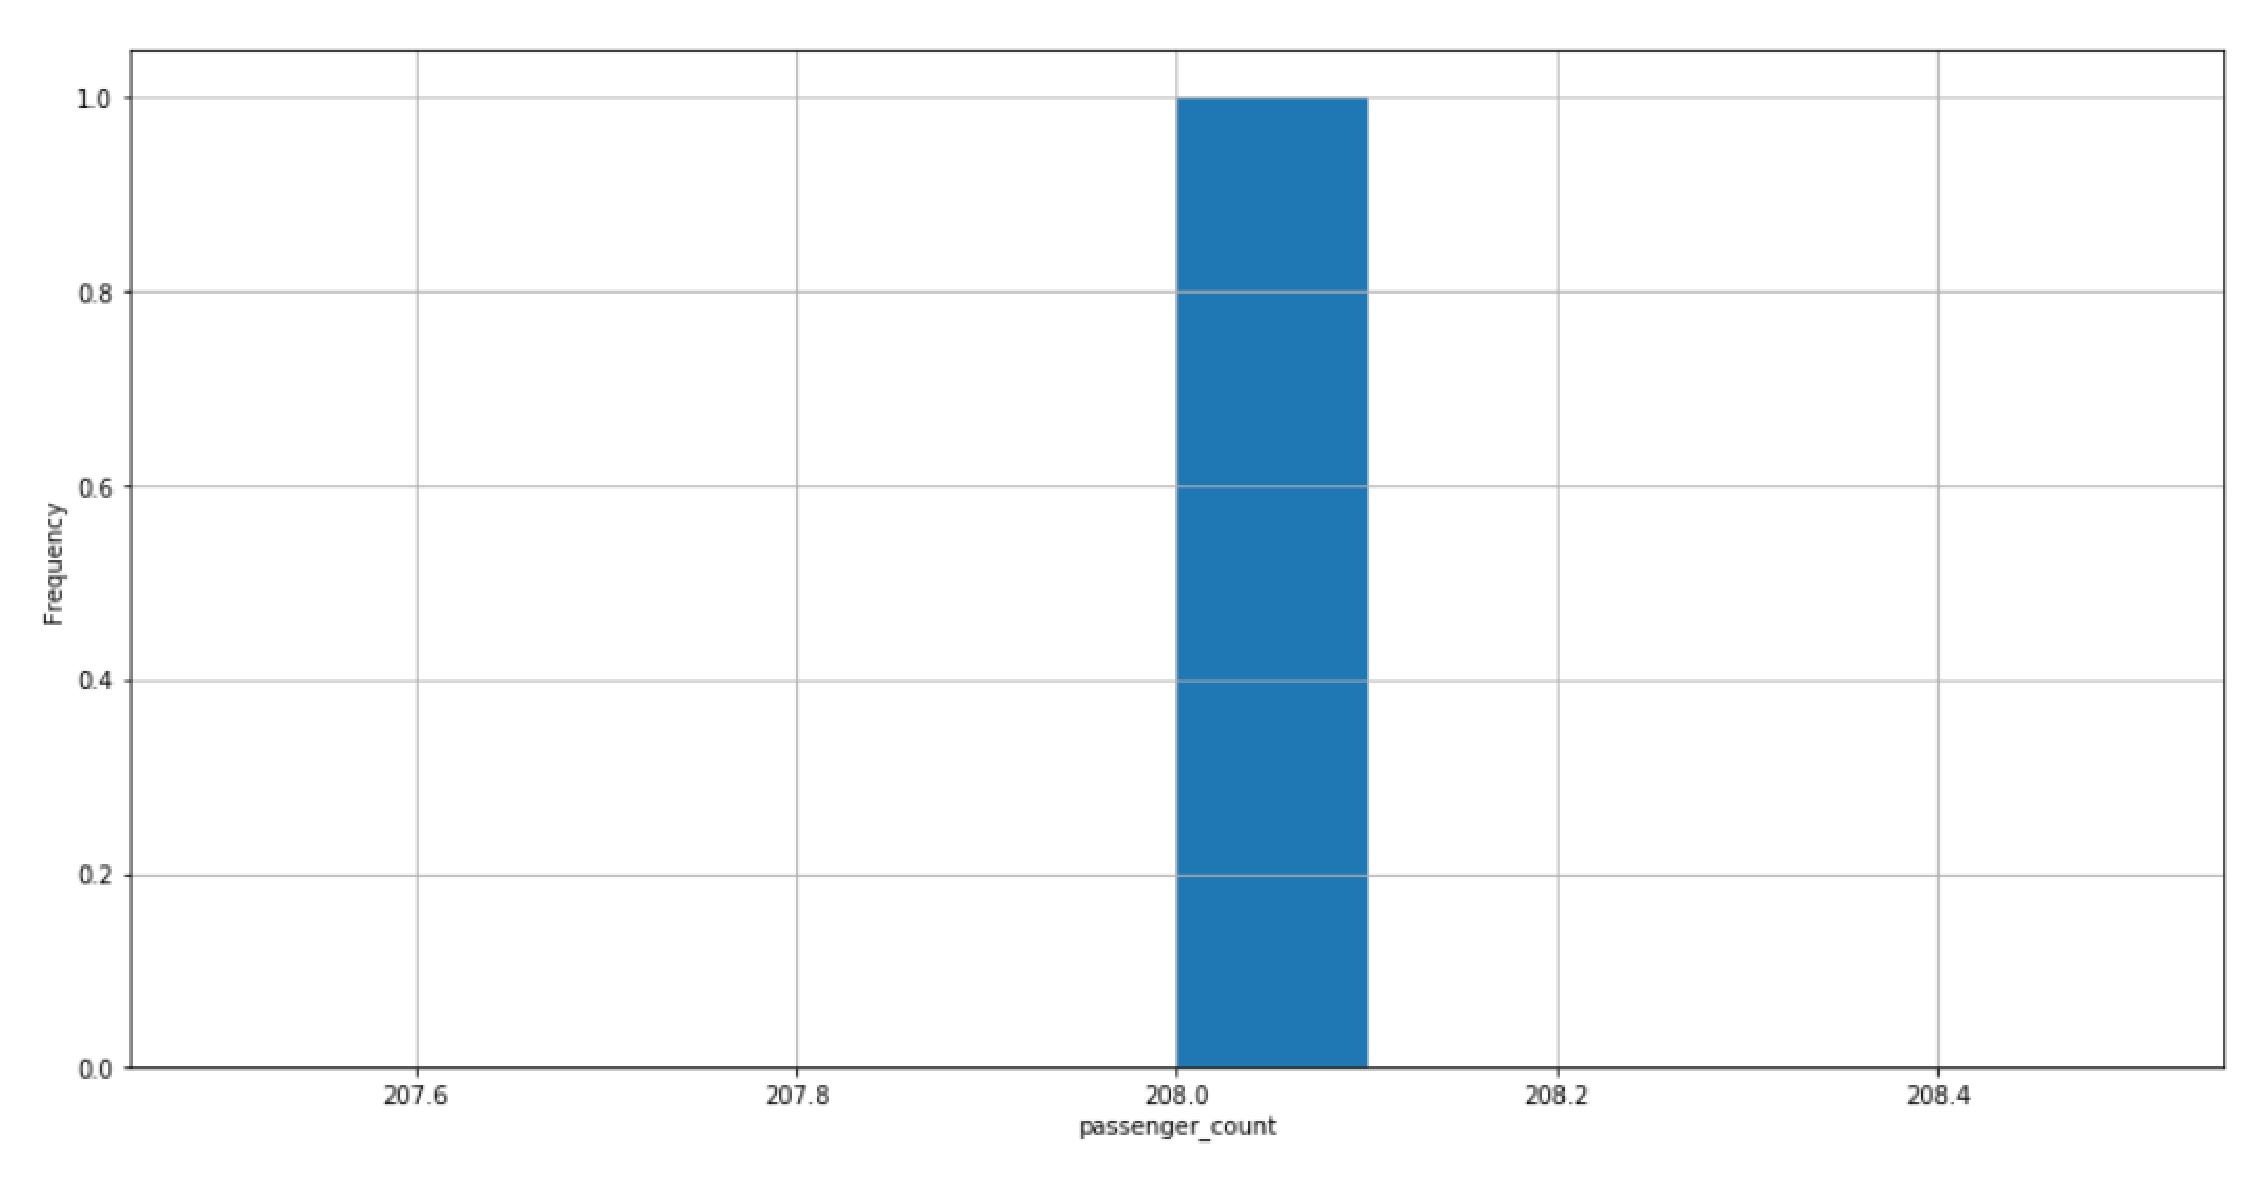
\includegraphics[scale=0.15]{3.eps}
        \end{minipage}
    }
    \caption{Histogram of different groups}
    \end{figure}
  % \begin{figure}[htbp]
  %     \centering
  %     \subfigure[$f_1$]
  %     {
  %       \begin{minipage}[b]{.3\linewidth}
  %         \centering
  %         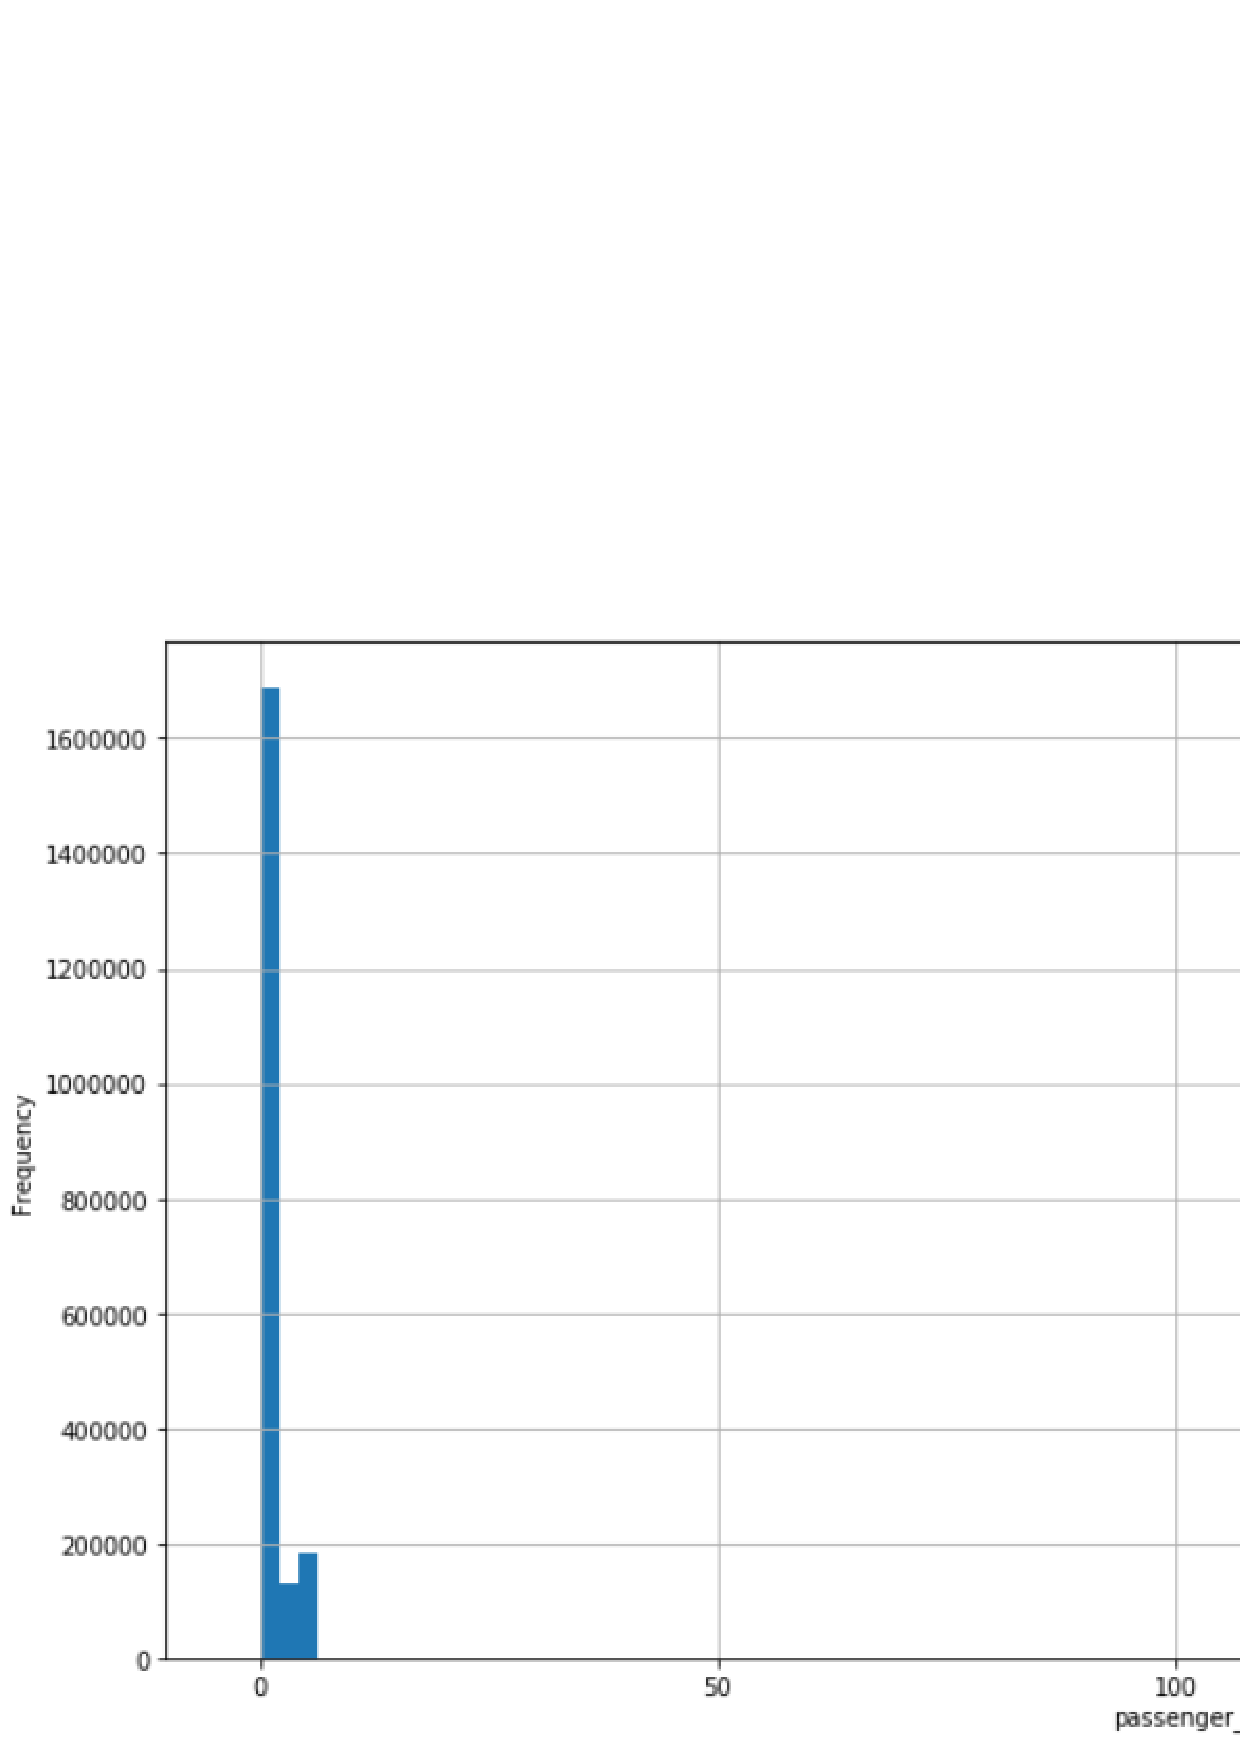
\includegraphics[scale=0.1]{1.png}
  %       \end{minipage}
  %         % \selectcolormodel{rgb}
  %         % \missingfigure[figwidth=5.5cm]{Test.}
  %         % %\includegraphics[width=0.25\textwidth]{figures//frequency-distribution-feature1.eps}
  %         % \label{fig:fre-dis-f1}
  %     }
  %     \subfigure[$f_2$]{
  %       \begin{minipage}[b]{.3\linewidth}
  %         \centering
  %         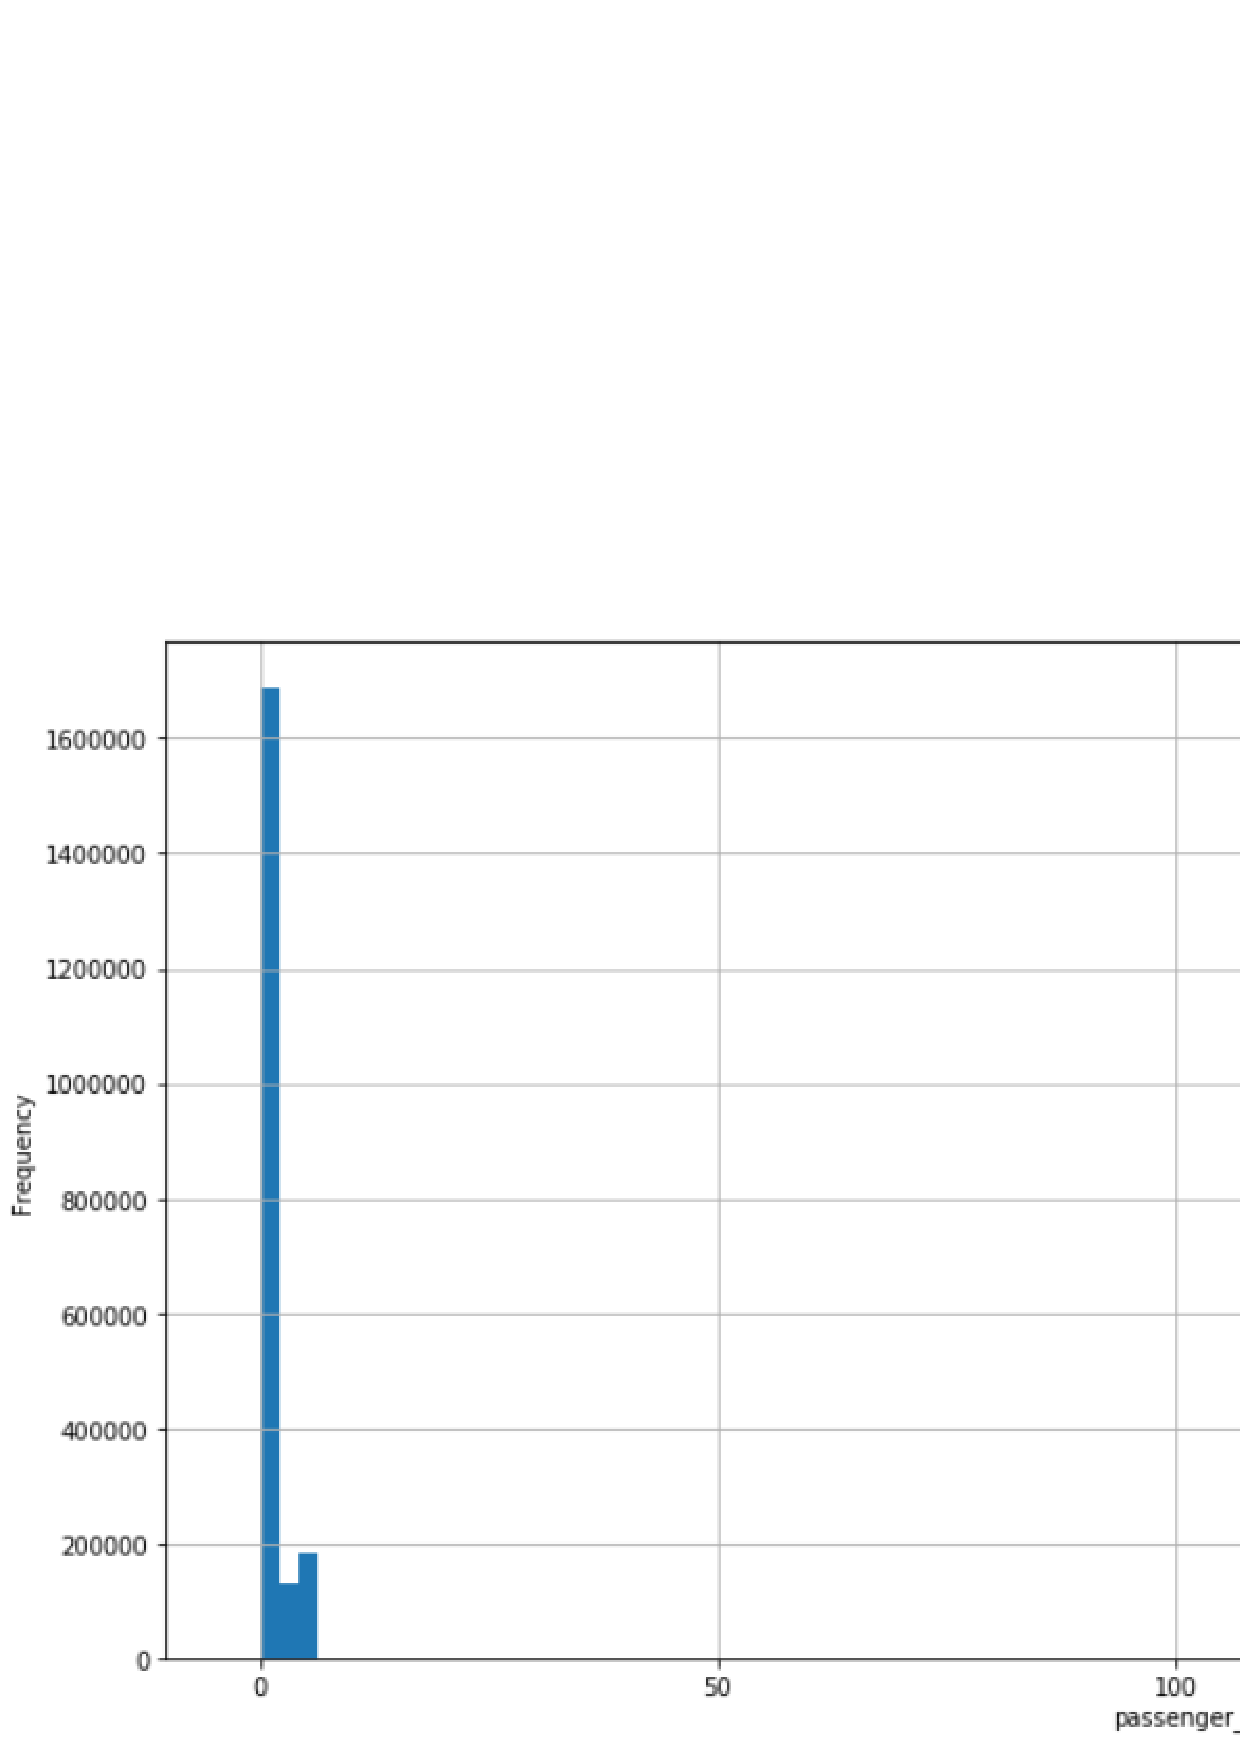
\includegraphics[scale=0.1]{1.png}
  %       \end{minipage}
  %         % \selectcolormodel{rgb}
  %         % \missingfigure[figwidth=5.5cm]{Test.}
  %         % \label{fig:fre-dis-f2}
  %     }
  %     \subfigure[$f_3$]{
  %       \begin{minipage}[b]{.3\linewidth}
  %         \centering
  %         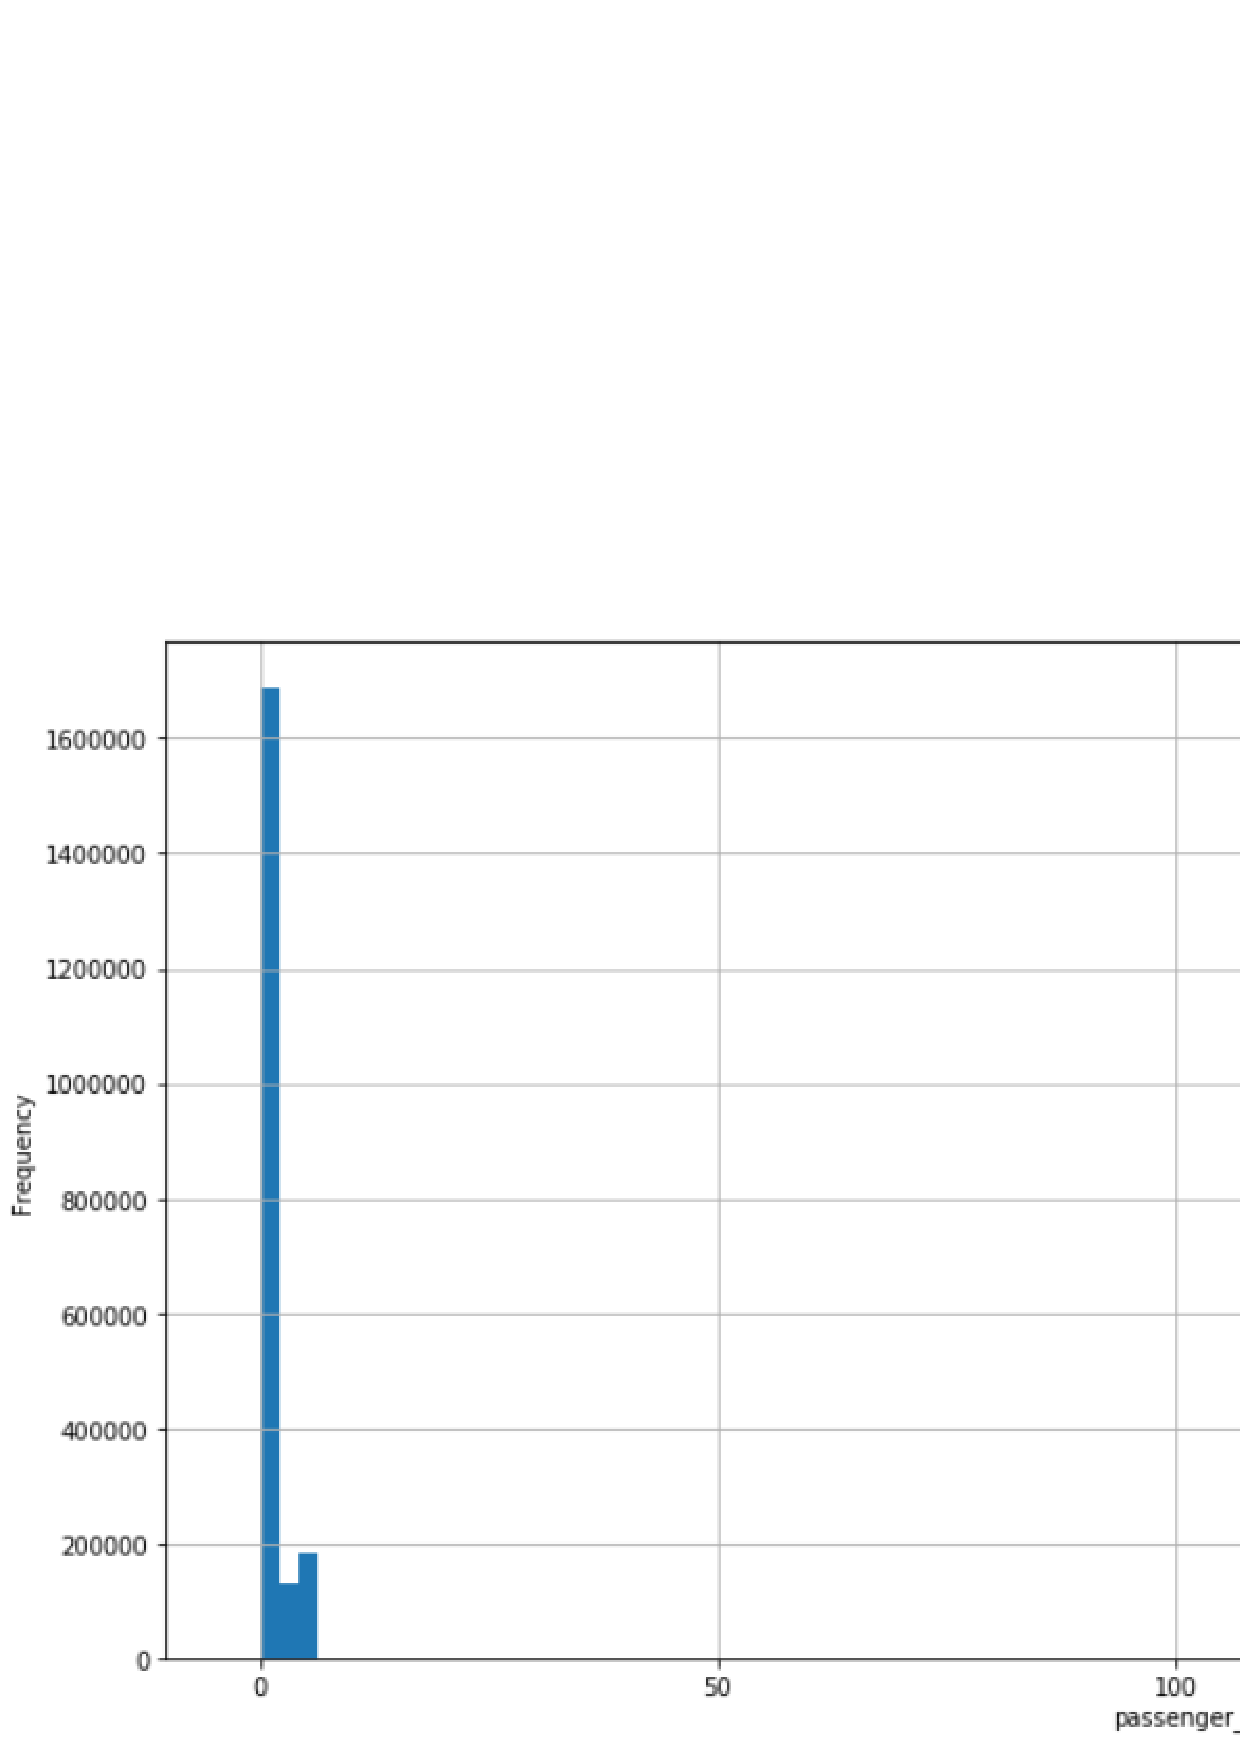
\includegraphics[scale=0.1]{1.png}
  %       \end{minipage}
  %     % \selectcolormodel{rgb}
  %         % \missingfigure[figwidth=5.5cm]{Test.}
  %         % \label{fig:fre-dis-f3}
  %     }
  %     \caption{Histogram of $G_q$ on three features}
  %     \label{fig:fre-dis-each-feature}
  % \end{figure}
  
  %%==========================================================================================
  \begin{note}
  Now, let me specifically explain what each step means.
  The first step is group feature extraction.
  we can take one group extraction as an example.
  
  We suppose to use $f_1$, $f_2$, $f_3$ to represent three features of $G_q$.
  The values of $f_1$ are {$x_1$, $x_2$, $x_3$, $x_4$} and so on.
  And the values of $f_2$ are {$y_2$, $y_2$, $y_1$, $x_2$} and so on.
  
  For feature $f_1$,
  we use the histogram to illustrate feature $f_1$ after
  counting the frequency of each value,
  as show in figure 6 (a).
  
  Similarly,
  we can also extract other features of the group
  according to feature $f_1$.
  \end{note}
  %%==========================================================================================
  
  \end{slide}
  %%
  %%==========================================================================================





%%==========================================================================================
%%
\begin{slide}{Processing and Computing}
  %Related Work - Outlying Aspects Mining
  \begin{itemize}
  \item
  Data processing and computing.
  
  
  \begin{itemize}
    \item
    Frame the training set range.Find the longitude and latitude range of the test set. The training dataset contains \textcolor{orange}{1957,917} records after being processed.
    \item
    Calculate the distance between pick-up and drop-off points according to the Haversine Equation.

    The records with zero distance between taxi fare and pick-up and drop-off location are invalid, and \textcolor{orange}{1957913} training set data are obtained after deletion.
    % \textcolor{orange}{Feature selection}
  \end{itemize}
  
  \end{itemize}
  
  
  
  %%==========================================================================================
  \begin{note}
  Let me introduce two existing methods:
  Feature selection and score-and-search.
  
  For feature selection,
  the query point can be regarded as positive class and
  the rest of the data can be regarded as negative class,
  selected the features that best distinguish the two classes.
  
  The advantages of this method are easy to operate,
  and it's able to resolve dimensionality bias.
  However, it has some drawbacks.
  Firstly,
  positive and negative classes are Not balanced,
  secondly,
  it can't quantify the outlying degree correctly.
  Most importantly,
  it doesn't identify group outlying aspects.
  \end{note}
  %%==========================================================================================
  
  \end{slide}
  %%
  %%==========================================================================================



\section{Data Modeling}
%%==========================================================================================
%%
\begin{slide}{Data Modeling}
  %Related Work - Outlying Aspects Mining
  \begin{itemize}
  \item
  Data modeling.
  
  \begin{itemize}
    \item
    multiple linear regression models matrix representation:$$
{Y} ={X}{\beta}+{\mu}$$

    The multiple regression equation is obtained as follows:$$
    \textcolor{orange}{{Y_i} =4.46+2.10{X_{0_i}}-0.05{X_{1_i}}+0.04{X_{2_i}}}
    $$where ${X_{0_i}}$ is the value of "H\_Distance", ${X_{1_i}}$ is the value of "weekday+1", ${X_{2_i}}$ is the value of "passenger\_count".
    % \textcolor{orange}{Feature selection}
  \end{itemize}
  
  \end{itemize}
  
  
  
  %%==========================================================================================
  \begin{note}
  Let me introduce two existing methods:
  Feature selection and score-and-search.
  
  For feature selection,
  the query point can be regarded as positive class and
  the rest of the data can be regarded as negative class,
  selected the features that best distinguish the two classes.
  
  The advantages of this method are easy to operate,
  and it's able to resolve dimensionality bias.
  However, it has some drawbacks.
  Firstly,
  positive and negative classes are Not balanced,
  secondly,
  it can't quantify the outlying degree correctly.
  Most importantly,
  it doesn't identify group outlying aspects.
  \end{note}
  %%==========================================================================================
  
  \end{slide}
  %%
  %%==========================================================================================



%%==========================================================================================
%%
\begin{slide}{Conclusion}
  %Related Work - Outlying Aspects Mining
  \begin{itemize}
  \item
  Data to predict.
  
  \begin{itemize}
    \item
    Putting the relevant fields of the prediction set into the regression equation yields the predicted value of "fare_amount" :

    \begin{table}  \centering
      \caption{Prediction for the field "fare\_amount"}
      \label{table:a}
      \begin{tabular}{ccc}
    \toprule
        % after \\: \hline or \cline{col1-col2} \cline{col3-col4} ...
        & key & fare\_amount \\
    \midrule
        0 & 2015-01-27 13:08:24.000000200 & 9.29 \\
        1 & 2015-01-27 13:08:24.000000300 & 9.50 \\
        2 & 2011-10-08 11:53:44.000000200 & 5.51 \\
        ... & ... &... \\
    \bottomrule
    \end{tabular}
    \end{table}
  
    % \textcolor{orange}{Feature selection}
  \end{itemize}
  
  \end{itemize}
  
  
  
  %%==========================================================================================
  \begin{note}
  Let me introduce two existing methods:
  Feature selection and score-and-search.
  
  For feature selection,
  the query point can be regarded as positive class and
  the rest of the data can be regarded as negative class,
  selected the features that best distinguish the two classes.
  
  The advantages of this method are easy to operate,
  and it's able to resolve dimensionality bias.
  However, it has some drawbacks.
  Firstly,
  positive and negative classes are Not balanced,
  secondly,
  it can't quantify the outlying degree correctly.
  Most importantly,
  it doesn't identify group outlying aspects.
  \end{note}
  %%==========================================================================================
  
  \end{slide}
  %%
  %%==========================================================================================
  



%   %%==========================================================================================
% %%
% \begin{slide}[toc=,bm=]{}
%   \twocolumn
%   {
%   \begin{itemize}
%   \item
%   \smallskip
%   \textcolor{orange}{Multiple} points.
%   \medskip
%   \end{itemize}
%   \vspace{0.75cm}
%   %\vspace{0.1cm}
%   \begin{figure}
%     % \begin{center}
%     %   \includegraphics[width=0.4\textwidth]{1passenger_count-10.png}
%     % \end{center}
%     \centering
%     \selectcolormodel{rgb}
%     \includegraphics[width=0.4\textwidth]{1passenger_count-10.png}
%     % \missingfigure{Testing a long text string.}
%     %\includegraphics[width=0.6\textwidth]{figures//example-basketball-projection.eps}\\
%     \caption{Group Outlying Aspects Target}\label{fig:GroupOutAspect-target}
%   \end{figure}
%   }

%   {
%   \begin{itemize}
  
%   \item
%   \textcolor{orange}{One} point.
%   \end{itemize}
%   \bigskip
%   \begin{figure}
%     % \begin{center}
%     %   \includegraphics[width=0.4\textwidth]{1passenger_count-10.png}
%     % \end{center}
%     \centering
%     \selectcolormodel{rgb}
%     \includegraphics[width=0.4\textwidth]{1passenger_count-10.png}
%     % \missingfigure{Testing a long text string.}
%     %\includegraphics[width=0.6\textwidth]{figures//example-basketball-projection.eps}\\
%     \caption{Outlying Aspects Target}\label{fig:OutAspect-target}
%   \end{figure}
%   }

% % \begin{slide}{}
% %   %Related Work - Outlying Aspects Mining
% %   \begin{figure}[h]
% %     \begin{center}
% %     \includegraphics[width=0.4\textwidth]{1passenger_count-10.png}
% %     \end{center}
% %     \caption{SJTU}
% %     \label{fig:a}
% %   \end{figure}
  
  
%   %%==========================================================================================
%   \begin{note}
%   Let me introduce two existing methods:
%   Feature selection and score-and-search.
  
%   For feature selection,
%   the query point can be regarded as positive class and
%   the rest of the data can be regarded as negative class,
%   selected the features that best distinguish the two classes.
  
%   The advantages of this method are easy to operate,
%   and it's able to resolve dimensionality bias.
%   However, it has some drawbacks.
%   Firstly,
%   positive and negative classes are Not balanced,
%   secondly,
%   it can't quantify the outlying degree correctly.
%   Most importantly,
%   it doesn't identify group outlying aspects.
%   \end{note}
%   %%==========================================================================================
  
%   \end{slide}
%   %%
%   %%==========================================================================================








%%==========================================================================================
% TODO: Contact Page
\begin{wideslide}[toc=,bm=]{Contact Information}
\centering
\vspace{\stretch{1}}
\twocolumn[
lcolwidth=0.35\linewidth,
rcolwidth=0.65\linewidth
]
{
% \centerline{\includegraphics[scale=.2]{tulip-logo.eps}}
}
{
\vspace{\stretch{1}}
Runsha Pan\\
School of Hunan University\\
\begin{description}
 \item[\textcolor{orange}{\faEnvelope}] \href{mailto:qq2724493252@163.com}
 {\textsc{\footnotesize{qq2724493252@163.com}}}

%  \item[\textcolor{orange}{\faHome}] \href{http://www.tulip.org.au}
%  {\textsc{\footnotesize{Team for Universal Learning and Intelligent Processing}}}
\end{description}
}
\vspace{\stretch{1}}
\end{wideslide}

\end{document}

\endinput
